\tikzstyle{input_neuron}=[circle,draw=black!100,fill=gray!80,thick,minimum size=6mm]
\tikzstyle{hidden_neuron}=[circle,draw=black!100,fill=white!100,thick,minimum size=6mm]
\tikzstyle{output_neuron}=[circle,draw=green!50,fill=green!10,thick,minimum size=6mm]

\tikzstyle{input}=[circle,draw=black!50,fill=black!20,thick,minimum size=6mm]

\begin{center}
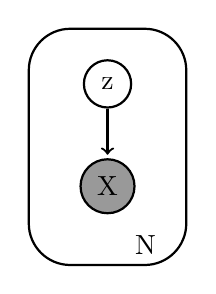
\begin{tikzpicture}
\node [input_neuron] (neuron51) at (7.5,6.5) {X} ;
\node [hidden_neuron] (neuron52) at (7.5,7.8)  {z};
\node[text width=0.1cm] at (7.9,5.75) {N};
\draw[black!100,thick,solid,rounded corners=15pt] (6.5,5.5) rectangle (8.5,8.5);
\draw[thick,->] (7.5,7.48) -- (7.5,6.9);
\end{tikzpicture}
\end{center}
